\documentclass[a4paper,12pt]{article}

\usepackage[utf8]{inputenc}
\usepackage[spanish]{babel}
\usepackage{amsmath, amssymb}
\usepackage{graphicx}
\usepackage{float}
\usepackage{booktabs}
\usepackage{xcolor}
\usepackage{listings}
\usepackage{caption}
\usepackage{fancyhdr}
\usepackage{hyperref}
\usepackage{tikz}
\usepackage{tabularx}

\hypersetup{
    colorlinks=true,
    linkcolor=blue,
    urlcolor=blue,
    pdftitle={Práctica 1 - Circuitos Combinacionales},
}

% === Definición de colores similares a Vivado ===
\definecolor{vivadoKeyword}{rgb}{0.6,0.0,0.6}
\definecolor{vivadoComment}{rgb}{0.0,0.5,0.0}
\definecolor{vivadoString}{rgb}{0.5,0.2,0.0}
\definecolor{vivadoBackground}{rgb}{0.97,0.97,0.97}

\lstdefinelanguage{VHDL}{
    morekeywords={library, use, entity, is, port, in, out, end, architecture, of, begin, signal, if, then, else, when, others, xor, and, or, not},
    sensitive=true,
    morecomment=[l]--,
    morestring=[b]",
}

\lstset{
    language=VHDL,
    backgroundcolor=\color{vivadoBackground},
    keywordstyle=\color{vivadoKeyword}\bfseries,
    commentstyle=\color{vivadoComment}\itshape,
    stringstyle=\color{vivadoString},
    basicstyle=\ttfamily\small,
    numbers=left,
    numberstyle=\tiny,
    numbersep=5pt,
    frame=single,
    breaklines=true,
    tabsize=2,
    captionpos=b
}

\title{Práctica N°3: Circuitos Secuenciales Regulares}
\date{}

\begin{document}
\maketitle
\tableofcontents
\newpage

\section{Objetivos}

\subsection{Objetivos Generales}
\begin{enumerate}
    \item Implementar un controlador de modulación por ancho de pulso (PWM) para el control de la potencia luminosa de un LED, aplicando técnicas de descripción de hardware.
\end{enumerate}

\subsection{Objetivos Específicos}
\begin{enumerate}
    \item Diseñar el circuito digital capaz de generar una señal PWM con ciclo de trabajo ajustable.
    \item Describir el circuito en un lenguaje de descripción de hardware (HDL) siguiendo las buenas prácticas de diseño.
    \item Simular el funcionamiento del controlador PWM para verificar el ajuste del brillo del LED.
    \item Implementar y probar el diseño en la tarjeta de desarrollo, validando el control de brillo en condiciones reales.
\end{enumerate}



\section{Descripción del Circuito en VHDL}

El diseño se ha dividido en tres módulos principales: \textbf{circuito PWM}, \textbf{Circuito Contador} y \textbf{Circuito Reset}.  
En esta sección se describe en detalle el primer bloque, encargado de generar la señal PWM (Pulse Width Modulation) cuyo ciclo de trabajo es ajustable mediante la entrada \texttt{duty\_cycle}. Este circuito se utiliza para controlar la potencia entregada a una carga, en este caso, un LED, variando el tiempo en que la señal permanece en alto durante cada periodo.

\subsection{Modulo 1: Circuito PWM}

Primero se presenta el código completo del modulo para posteriormente analizar cada parámetro relevantes.

\newpage

\begin{lstlisting}[caption={Código completo del módulo PWM}, label={lst:pwm_full}]
library ieee;
use ieee.std_logic_1164.all;
use ieee.numeric_std.all;

entity pwm is
  generic (
    pwm_bits : integer;
    clk_cnt_len : positive := 1
  );
  port (
    clk        : in std_logic;
    rst        : in std_logic;
    duty_cycle : in unsigned (pwm_bits - 1 downto 0);
    pwm_out    : out std_logic
  );
end pwm;

architecture rtl of pwm is
  signal pwm_cnt : unsigned (pwm_bits - 1 downto 0);
  signal clk_cnt : integer range 0 to clk_cnt_len - 1;
begin
  PWM_PROC : process( clk )
  begin
    if rising_edge(clk) then
      if rst = '1' then
        pwm_cnt <= (others => '0');
        pwm_out <= '0';
      else
        if clk_cnt_len = 1 or clk_cnt = 0 then
          pwm_cnt <= pwm_cnt + 1; -- contador infinito
          pwm_out <= '0';

          if pwm_cnt = unsigned(to_signed(-2, pwm_cnt'length)) then
            pwm_cnt <= (others => '0');
          end if;

          if pwm_cnt < duty_cycle then
            pwm_out <= '1';
          end if;
        end if;
      end if;
    end if;
  end process; 

  CLK_CNT_PROC : process( clk )
  begin
    if rising_edge(clk) then
      if rst = '1' then
        clk_cnt <= 0;
      else
        if clk_cnt < clk_cnt_len - 1 then
          clk_cnt <= clk_cnt + 1;
        else
          clk_cnt <= 0;
        end if;
      end if;
    end if;
  end process; 
end architecture;
\end{lstlisting}


\subsubsection*{Definición de la Entidad y Parámetros}

En primer lugar, se declara la entidad \texttt{pwm}, la cual incluye parámetros genéricos para definir la resolución de la señal y la división de frecuencia:



\begin{lstlisting}[caption={Entidad del módulo PWM}, label={lst:pwm_entity}]
library ieee;
use ieee.std_logic_1164.all;
use ieee.numeric_std.all;

entity pwm is
  generic (
    pwm_bits : integer;
    clk_cnt_len : positive := 1
  );
  port (
    clk        : in std_logic;
    rst        : in std_logic;
    duty_cycle : in unsigned (pwm_bits - 1 downto 0);
    pwm_out    : out std_logic
  );
end pwm;
\end{lstlisting}

El parámetro \texttt{pwm\_bits} define el número de bits del contador principal, lo que determina la resolución del PWM. El parámetro \texttt{clk\_cnt\_len} permite implementar un prescaler para reducir la frecuencia de la señal de reloj utilizada en la generación del PWM.

\subsubsection*{Arquitectura y Señales Internas}

Dentro de la arquitectura \texttt{rtl}, se definen dos señales internas: 

\begin{itemize}
    \item \texttt{pwm\_cnt}: contador principal que determina el ciclo de trabajo.
    \item \texttt{clk\_cnt}: contador auxiliar para dividir la frecuencia del reloj.
\end{itemize}

\begin{lstlisting}[caption={Definición de señales internas}, label={lst:pwm_signals}]
architecture rtl of pwm is
  signal pwm_cnt : unsigned (pwm_bits - 1 downto 0);
  signal clk_cnt : integer range 0 to clk_cnt_len - 1;
\end{lstlisting}

\subsubsection*{Proceso de Generación de PWM}

El proceso \texttt{PWM\_PROC} es el encargado de incrementar el contador principal y generar la señal PWM. Cuando \texttt{pwm\_cnt} es menor que \texttt{duty\_cycle}, la salida se coloca en alto, generando el pulso correspondiente.

\begin{lstlisting}[caption={Proceso de generación de PWM}, label={lst:pwm_proc}]
PWM_PROC : process( clk )
begin
  if rising_edge(clk) then
    if rst = '1' then
      pwm_cnt <= (others => '0');
      pwm_out <= '0';
    else
      if clk_cnt_len = 1 or clk_cnt = 0 then
        pwm_cnt <= pwm_cnt + 1;
        pwm_out <= '0';

        if pwm_cnt = unsigned(to_signed(-2, pwm_cnt'length)) then
          pwm_cnt <= (others => '0');
        end if;

        if pwm_cnt < duty_cycle then
          pwm_out <= '1';
        end if;
      end if;
    end if;
  end if;
end process;
\end{lstlisting}

En este bloque se observa:
\begin{enumerate}
    \item Reinicio del contador y salida cuando \texttt{rst} está activo.
    \item Incremento del contador \texttt{pwm\_cnt} en cada ciclo válido.
    \item Comparación con el valor de \texttt{duty\_cycle} para encender o apagar la salida.
\end{enumerate}

\subsubsection*{Proceso de División de Reloj}

El proceso \texttt{CLK\_CNT\_PROC} se utiliza como prescaler. Esto permite ajustar la frecuencia del PWM sin modificar la frecuencia de reloj principal.


\begin{lstlisting}[caption={Proceso de división de reloj}, label={lst:clk_cnt_proc}]
CLK_CNT_PROC : process( clk )
begin
  if rising_edge(clk) then
    if rst = '1' then
      clk_cnt <= 0;
    else
      if clk_cnt < clk_cnt_len - 1 then
        clk_cnt <= clk_cnt + 1;
      else
        clk_cnt <= 0;
      end if;
    end if;
  end if;
end process;
\end{lstlisting}

Este prescaler es especialmente útil para evitar que la señal PWM tenga una frecuencia demasiado alta, lo que podría impedir la correcta percepción del cambio de brillo en el LED.


\subsection{Modulo 2: Circuito Contador}

Este módulo implementa un contador genérico que incrementa su valor en cada flanco ascendente del reloj cuando la señal \texttt{count\_enable} está activa. El contador es auto envolvente, lo que significa que cuando alcanza su valor máximo, vuelve a cero automáticamente. El rango máximo depende del número de bits especificado por el parámetro genérico.

\subsubsection{Código VHDL Completo del Contador}

\begin{lstlisting}[caption={Código completo del módulo Contador}, label={lst:counter_full}]
library ieee;
use ieee.std_logic_1164.all;
use ieee.numeric_std.all;
use ieee.math_real.all;

entity counter is
  generic (
    counter_bits : integer
  );
  port (
    clk          : in std_logic;
    rst          : in std_logic;
    count_enable : in std_logic;
    counter      : out unsigned (counter_bits - 1 downto 0)
  );
end counter;

architecture rtl of counter is
  signal counter_i : unsigned(counter'range);
begin

  counter <= counter_i;

  COUNTER_PROC : process(clk)
  begin
    if rising_edge(clk) then  
      if rst = '1' then
        counter_i <= (others => '0');
      else
        if count_enable = '1' then
          counter_i <= counter_i + 1;
        end if ;
      end if ;
    end if ;
  end process;
end architecture;
\end{lstlisting}

\subsubsection{Definición de la Entidad y Parámetro Genérico}

\begin{lstlisting}[caption={Entidad del módulo Contador}, label={lst:counter_entity}]
entity counter is
  generic (
    counter_bits : integer
  );
  port (
    clk          : in std_logic;
    rst          : in std_logic;
    count_enable : in std_logic;
    counter      : out unsigned (counter_bits - 1 downto 0)
  );
end counter;
\end{lstlisting}

En esta entidad se define:
\begin{itemize}
    \item \textbf{counter\_bits}: parámetro genérico que establece el número de bits del contador, determinando su rango máximo.
    \item \textbf{clk}: señal de reloj.
    \item \textbf{rst}: señal de reinicio síncrono que pone el contador en cero.
    \item \textbf{count\_enable}: habilitador que permite o detiene la cuenta.
    \item \textbf{counter}: salida del valor actual del contador.
\end{itemize}

\subsubsection{Señales Internas}

Dentro de la arquitectura se define una señal interna \texttt{counter\_i}, que almacena el valor actual del contador y se asigna continuamente a la salida \texttt{counter}.

\begin{lstlisting}[caption={Definición de señal interna del contador}, label={lst:counter_signal}]
signal counter_i : unsigned(counter'range);
\end{lstlisting}

\subsubsection{Proceso de Conteo}

El proceso \texttt{COUNTER\_PROC} se activa en cada flanco ascendente del reloj. Si la señal \texttt{rst} está activa, el contador se reinicia a cero. Si \texttt{count\_enable} está en alto, el valor del contador se incrementa en una unidad.

\begin{lstlisting}[caption={Proceso de conteo}, label={lst:counter_proc}]
COUNTER_PROC : process(clk)
begin
  if rising_edge(clk) then  
    if rst = '1' then
      counter_i <= (others => '0');
    else
      if count_enable = '1' then
        counter_i <= counter_i + 1;
      end if ;
    end if ;
  end if ;
end process;
\end{lstlisting}

Este mecanismo permite implementar fácilmente contadores de diferente tamaño ajustando únicamente el parámetro \texttt{counter\_bits}, sin modificar el resto del código.


\subsection{Modulo 3: Circuito Reset}

Este módulo implementa un circuito de \textit{reset} sincronizado y filtrado, encargado de generar una señal de reinicio interno (\texttt{rst}) a partir de una señal externa (\texttt{rst\_n}). Su función es garantizar que el reinicio del sistema ocurra de forma controlada, evitando activaciones indeseadas provocadas por rebotes o inestabilidades en la señal externa.

\newpage

\subsubsection{Código VHDL Completo del Circuito Reset}

\begin{lstlisting}[caption={Código completo del módulo Reset}, label={lst:reset_full}]
library ieee;
use ieee.std_logic_1164.all;
use ieee.numeric_std.all;

entity reset is
  port (
    clk : in std_logic;
    rst_n : in std_logic; 
    rst : out std_logic
  );
end reset;

architecture rtl of reset is

  signal sreg : std_logic_vector(3 downto 0);

begin
  SREG_PROC : process(clk)
  begin
    if rising_edge(clk) then
      sreg <= sreg(sreg'high - 1 downto 0) & rst_n;
    end if ;
  end process;

  RESET_PROC : process(sreg)
    constant all_ones : std_logic_vector(sreg'range) := (others => '1');
  begin
    if sreg = all_ones then
      rst <= '0';
    else
      rst <= '1';
    end if ;
  end process;

end architecture;
\end{lstlisting}

\newpage

\subsubsection{Definición de la Entidad}

\begin{lstlisting}[caption={Entidad del módulo Reset}, label={lst:reset_entity}]
entity reset is
  port (
    clk : in std_logic;
    rst_n : in std_logic; 
    rst : out std_logic
  );
end reset;
\end{lstlisting}

En esta entidad:
\begin{itemize}
    \item \textbf{clk}: señal de reloj utilizada para sincronizar el filtrado del reset.
    \item \textbf{rst\_n}: señal externa de reset, activa en bajo.
    \item \textbf{rst}: señal de reset interno, activa en alto.
\end{itemize}

\subsubsection{Señales Internas}

El módulo emplea un registro de desplazamiento (\texttt{sreg}) de 4 bits para filtrar y estabilizar la señal de entrada. Esto permite que la señal de reset interno solo se desactive cuando la entrada externa se haya mantenido estable por varios ciclos de reloj.

\begin{lstlisting}[caption={Registro de desplazamiento para filtrado}, label={lst:reset_signal}]
signal sreg : std_logic_vector(3 downto 0);
\end{lstlisting}

\subsubsection{Proceso de Registro de Desplazamiento}

El proceso \texttt{SREG\_PROC} captura el estado de la señal \texttt{rst\_n} en cada flanco ascendente del reloj y lo va desplazando dentro del registro \texttt{sreg}. Esto actúa como un filtro contra cambios rápidos o inestables.

\begin{lstlisting}[caption={Proceso de desplazamiento de la señal rst\_n}, label={lst:sreg_proc}]
SREG_PROC : process(clk)
begin
  if rising_edge(clk) then
    sreg <= sreg(sreg'high - 1 downto 0) & rst_n;
  end if ;
end process;
\end{lstlisting}

\subsubsection{Proceso de Generación de la Señal Reset Interna}

El proceso \texttt{RESET\_PROC} compara el contenido del registro \texttt{sreg} con un vector de todos unos (\texttt{all\_ones}).  
\begin{itemize}
    \item Si todos los bits son ‘1’, significa que la señal externa \texttt{rst\_n} ha estado en alto de forma estable, y por lo tanto se libera el reset interno (\texttt{rst} = ‘0’).
    \item En cualquier otro caso, el reset interno permanece activo (\texttt{rst} = ‘1’).
\end{itemize}

\begin{lstlisting}[caption={Proceso de generación del reset interno}, label={lst:reset_proc}]
RESET_PROC : process(sreg)
  constant all_ones : std_logic_vector(sreg'range) := (others => '1');
begin
  if sreg = all_ones then
    rst <= '0';
  else
    rst <= '1';
  end if ;
end process;
\end{lstlisting}




\subsection{Archivo principal}

En este módulo de nivel superior se integran los tres bloques: \texttt{PWM}, \texttt{Contador} y \texttt{Reset}. La idea es usar una onda de sierra (producida por el contador) para formar el \textit{duty cycle} del PWM y, con ello, variar el brillo de un LED. La señal \texttt{count\_enable} del contador se fija en \texttt{'1'} para evitar errores de uso y asegurar el conteo continuo.

\newpage

\subsubsection{Código VHDL completo del nivel superior}

\begin{lstlisting}[caption={Archivo principal: integración de PWM, contador y reset}, label={lst:top_full}]
library ieee;
use ieee.std_logic_1164.all;
use ieee.numeric_std.all;

-- Entidad principal: integra PWM, contador y circuito de reset
entity pwm_led is
  generic(
    -- Resolucion del PWM en bits; define los niveles de duty cycle
    pwm_bits : integer := 8;

    -- Prescaler interno del PWM (divide el reloj)
    -- Frecuencia del PWM (aprox):
    --   f_pwm = f_clk / ((2^pwm_bits - 1) * clk_cnt_len)
    -- Ejemplo con f_clk = 100 MHz:
    --   f_pwm = 100e6 / ( (255) * 392 ) = 1000.4 Hz
    clk_cnt_len : positive := 392;

    -- Ancho del contador que genera la onda de sierra (duty base)
    -- Frecuencia de la sierra (envolvente):
    --   f_saw = f_clk / 2^cnt_bits
    -- Para f_clk = 100 MHz y cnt_bits = 28:
    --   f_saw = 100e6 / 268,435,456 = 0.37 Hz (periodo = 2.68 s)
    -- Ojo: a veces se escribe al reves; esta es la relacion correcta.
    cnt_bits : integer := 28
  );
  port (
    clk   : in std_logic;  -- Reloj del sistema
    rst_n : in std_logic;  -- Reset externo activo en bajo (pull-up)
    led   : out std_logic  -- Salida al LED
  );
end pwm_led;

architecture rtl of pwm_led is
  -- Senales internas
  signal rst     : std_logic;                            -- Reset sincronizado/filtrado
  signal cnt     : unsigned (cnt_bits - 1 downto 0);     -- Contador principal (sierra)
  signal pwm_out : std_logic;                            -- Salida PWM

  -- Alias: toma los 'pwm_bits' mas significativos de 'cnt' como duty_cycle del PWM.
  -- Esto produce una rampa de duty entre 0 y (2^pwm_bits - 1) que se repite
  -- a la velocidad de la sierra (f_saw).
  alias duty_cycle is cnt(cnt'high downto cnt'length - pwm_bits);

begin
  -- El LED sigue directamente la salida del PWM
  led <= pwm_out;

  -- 1) Reset: sincroniza y filtra rst_n para generar 'rst' activo en alto
  RESET : entity work.reset(rtl)
    port map(
      clk   => clk,
      rst_n => rst_n,
      rst   => rst
    );

  -- 2) PWM: genera la senal PWM con duty definido por los bits altos de 'cnt'
  PWM : entity work.pwm(rtl)
    generic map (
      pwm_bits    => pwm_bits,
      clk_cnt_len => clk_cnt_len
    )
    port map (
      clk        => clk,
      rst        => rst,
      duty_cycle => duty_cycle,
      pwm_out    => pwm_out
    );

  -- 3) Contador: produce la sierra. Habilitado permanentemente (count_enable = '1')
  COUNTER : entity work.counter(rtl)
    generic map (
      counter_bits => cnt'length
    )
    port map (
      clk          => clk,
      rst          => rst,
      count_enable => '1',  -- Conteo continuo (evita errores de usuario)
      counter      => cnt
    );
end architecture;
\end{lstlisting}

\subsubsection{Análisis de parámetros y diseño}

\paragraph{Genéricos del nivel superior}
\begin{itemize}
  \item \textbf{\texttt{pwm\_bits}}: resolución del \textit{duty}. A mayor valor, transición de brillo más suave.
  \item \textbf{\texttt{clk\_cnt\_len}}: prescaler del PWM. Aumentarlo reduce la frecuencia del PWM (útil para no exceder la respuesta de la carga).
  \item \textbf{\texttt{cnt\_bits}}: controla la velocidad de la rampa (sierra). Con \(f_\text{clk}=100\,\text{MHz}\), \(f_\text{saw}=f_\text{clk}/2^{\text{cnt\_bits}}\). 
\end{itemize}

\paragraph{Señales internas y alias}
\begin{itemize}
  \item \textbf{\texttt{cnt}}: contador libre que da la forma de onda base (sierra).
  \item \textbf{\texttt{duty\_cycle}} (alias): toma los bits más altos de \texttt{cnt} para generar un duty proporcional al valor instantáneo de la sierra.
  \item \textbf{\texttt{rst}}: reset interno sincronizado, activo en alto, derivado de \texttt{rst\_n}.
\end{itemize}

\paragraph{Flujo de datos}
\begin{enumerate}
  \item \texttt{counter} incrementa \texttt{cnt} (sierra).
  \item El alias \texttt{duty\_cycle} extrae los \texttt{pwm\_bits} más altos de \texttt{cnt}.
  \item \texttt{pwm} compara \texttt{pwm\_cnt} vs \texttt{duty\_cycle} y produce \texttt{pwm\_out}.
  \item \texttt{led} sigue \texttt{pwm\_out}.
\end{enumerate}



\section{Diagrama de Bloques}

En esta sección se presenta el diagrama de bloques del módulo principal \texttt{pwm\_led} y los submódulos que lo componen.  
Cada bloque representa una entidad VHDL independiente que cumple una función específica dentro del sistema general.

\subsection{Diagrama General del Módulo Principal}

\begin{figure}[H]
    \centering
    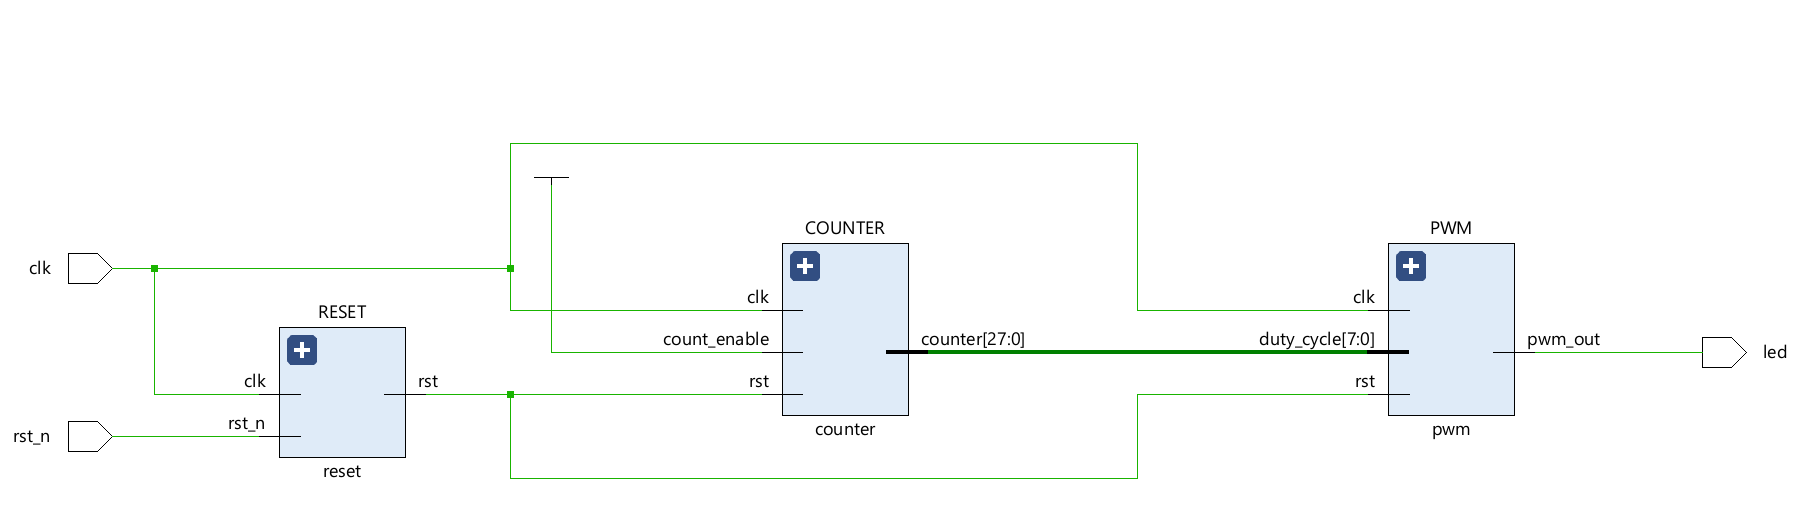
\includegraphics[width=0.85\textwidth]{Esquematicos/Top.png}
    \caption{Diagrama de bloques del módulo principal \texttt{pwm\_led}.}
    \label{fig:diagrama_pwm_led}
\end{figure}

El módulo principal integra tres submódulos:
\begin{itemize}
    \item \textbf{RESET}: Se encarga de generar una señal de reinicio controlada a partir de la entrada \texttt{rst\_n}.
    \item \textbf{COUNTER}: Genera una onda de sierra mediante un contador binario ascendente.
    \item \textbf{PWM}: Convierte la señal de onda de sierra en una señal de modulación por ancho de pulso (PWM) para controlar el brillo del LED.
\end{itemize}

\subsection{Módulo RESET}

\begin{figure}[H]
    \centering
    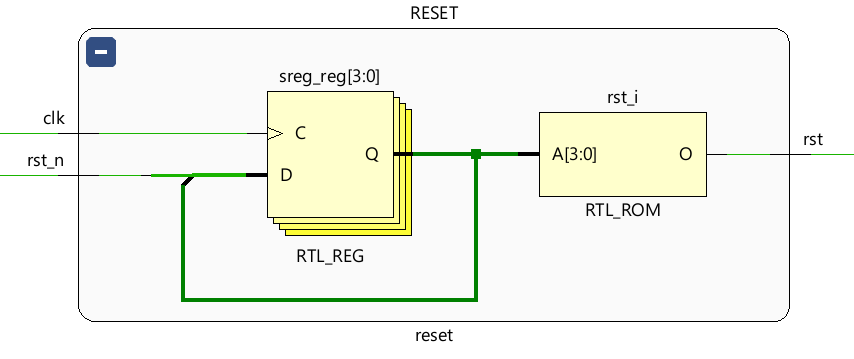
\includegraphics[width=0.85\textwidth]{Esquematicos/reset.png}
    \caption{Bloque funcional del módulo \texttt{RESET}.}
    \label{fig:diagrama_reset}
\end{figure}

Este módulo recibe la señal de reloj \texttt{clk} y la señal de reinicio activa en bajo \texttt{rst\_n}.  
Internamente utiliza un registro de desplazamiento para filtrar rebotes o ruidos, asegurando que la salida \texttt{rst} sea estable antes de iniciar el resto del sistema.

\subsection{Módulo COUNTER}

\begin{figure}[H]
    \centering
    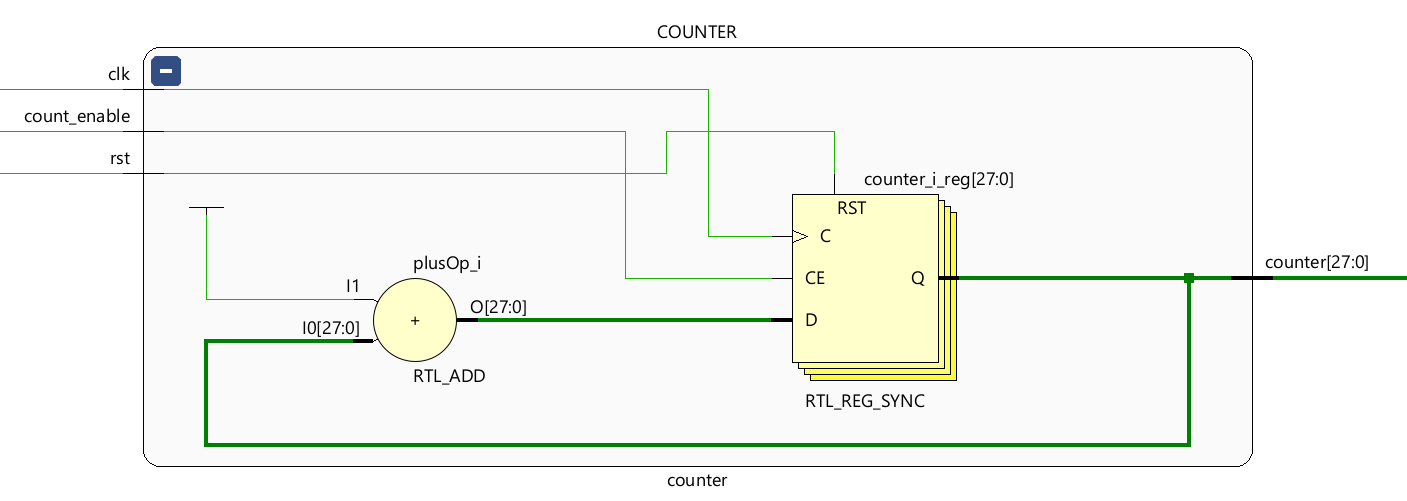
\includegraphics[width=0.85\textwidth]{Esquematicos/counter.png}
    \caption{Bloque funcional del módulo \texttt{COUNTER}.}
    \label{fig:diagrama_counter}
\end{figure}

Este módulo es un contador binario ascendente que genera una onda de sierra digital.  
Su frecuencia de incremento está determinada por la señal de reloj \texttt{clk} y el número de bits de conteo.  
La salida \texttt{cnt} se usa para determinar el ciclo de trabajo (\texttt{duty\_cycle}) del PWM.

\subsection{Módulo PWM}

\begin{figure}[H]
    \centering
    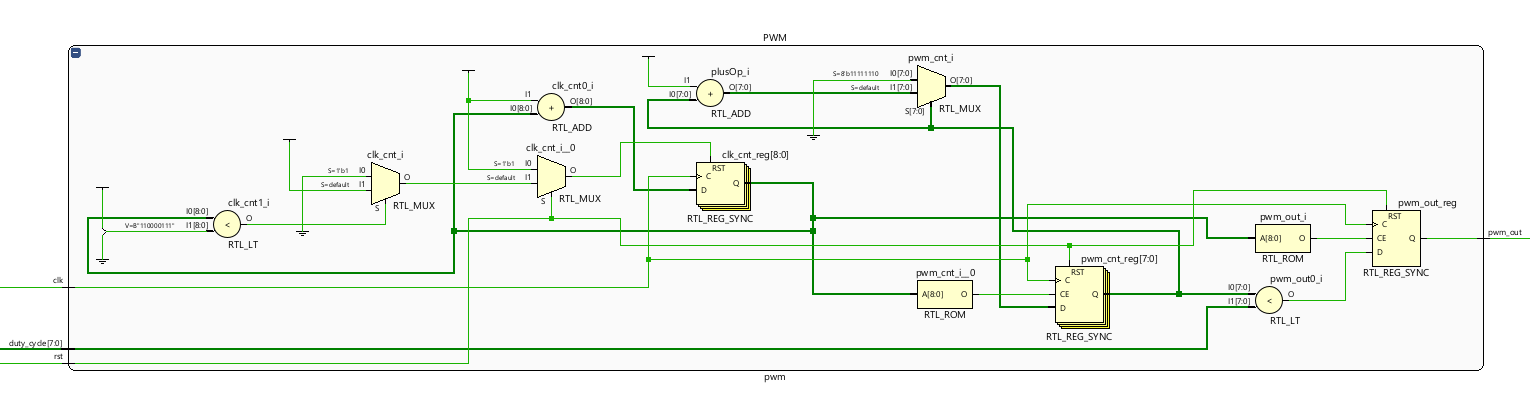
\includegraphics[width=0.85\textwidth]{Esquematicos/pwm.png}
    \caption{Bloque funcional del módulo \texttt{PWM}.}
    \label{fig:diagrama_pwm}
\end{figure}

Este módulo compara el valor del \texttt{duty\_cycle} con un contador interno para generar una señal PWM.  
Cuando el contador es menor que el ciclo de trabajo, la salida \texttt{pwm\_out} se mantiene en alto; de lo contrario, se pone en bajo.  
Esto permite controlar el brillo del LED dependiendo del tiempo que la señal se mantenga activa en cada ciclo.




\section{Asignación de Pines en la Nexys A7-100T}

Para la implementación en la tarjeta \textbf{Nexys A7-100T} se requiere definir las conexiones físicas entre las señales del diseño VHDL y los pines del FPGA.  
La \textbf{asignación de pines} se realiza en el archivo de restricciones \texttt{.xdc} y permite garantizar que cada señal se conecte al componente físico correcto de la placa.

En este proyecto se utilizan únicamente tres señales: el reloj (\texttt{CLK}), la señal de reinicio activo bajo (\texttt{RST\_n}) y la salida hacia el LED (\texttt{LED\_OUT}).

\begin{table}[H]
    \centering
    \renewcommand{\arraystretch}{1.2}
    \begin{tabularx}{0.75\textwidth}{|c|c|X|}
        \hline
        \textbf{Señal} & \textbf{Pin FPGA} & \textbf{Descripción} \\ \hline
        \texttt{CLK} & E3 & Entrada de reloj principal de 100\,MHz que provee la Nexys A7. \\ \hline
        \texttt{RST\_n} & J15 & Pulsador de usuario conectado con lógica activa en bajo, usado para reiniciar el sistema. \\ \hline
        \texttt{LED\_OUT} & H17 & LED de usuario en la parte superior derecha, usado para visualizar la señal PWM generada. \\ \hline
    \end{tabularx}
    \caption{Asignación de pines en la Nexys A7-100T.}
    \label{tab:asignacion_pines}
\end{table}

\subsection*{Justificación de la selección de pines}
\begin{itemize}
    \item \textbf{CLK (E3):} Este pin está cableado internamente al oscilador de 100\,MHz de la placa, por lo que es la opción estándar para el reloj del sistema.
    \item \textbf{RST\_n (J15):} Se elige este pin porque corresponde a uno de los switch de usuario (\texttt{SW0}).
    \item \textbf{LED\_OUT (H17):} Este pin controla uno de los LEDs de usuario, permitiendo observar visualmente el resultado del PWM en tiempo real.
\end{itemize}

\section{Resultados en la Placa Nexys A7 100T}

Para validar el funcionamiento del diseño implementado en la \textbf{Nexys A7-100T}, se realizaron pruebas prácticas observando el comportamiento del LED de salida (\texttt{LED\_OUT}) al cambiar el estado del interruptor asociado a la señal \texttt{RST\_n}.

\subsection*{Caso 1: Switch en bajo (sin salida)}
En este estado, el interruptor de entrada se mantiene en posición baja.  
El sistema permanece en reposo y el LED \texttt{LED\_OUT} se mantiene apagado.

\begin{figure}[H]
    \centering
    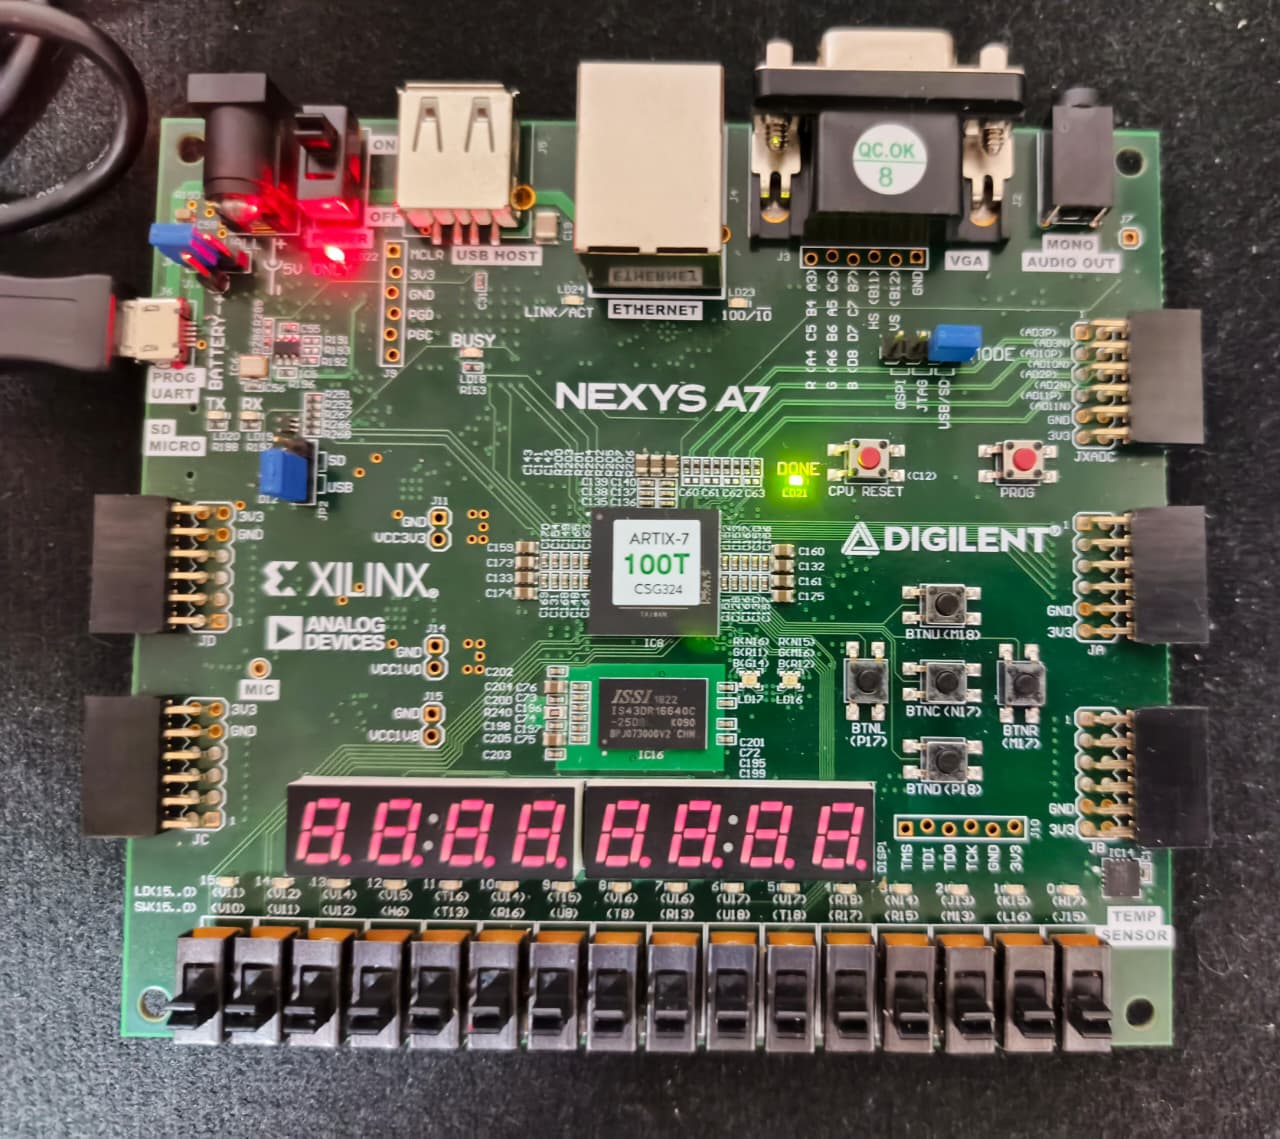
\includegraphics[width=0.6\textwidth]{Resultados/Salida_bajo.jpg}
    \caption{Switch en bajo: sin señal de salida, LED apagado.}
    \label{fig:switch_bajo}
\end{figure}

\subsection*{Caso 2: Switch en alto (LED encendido)}
Cuando el interruptor pasa a estado alto, el sistema activa la salida y el LED correspondiente se enciende, confirmando el funcionamiento correcto de la lógica implementada.

\begin{figure}[H]
    \centering
    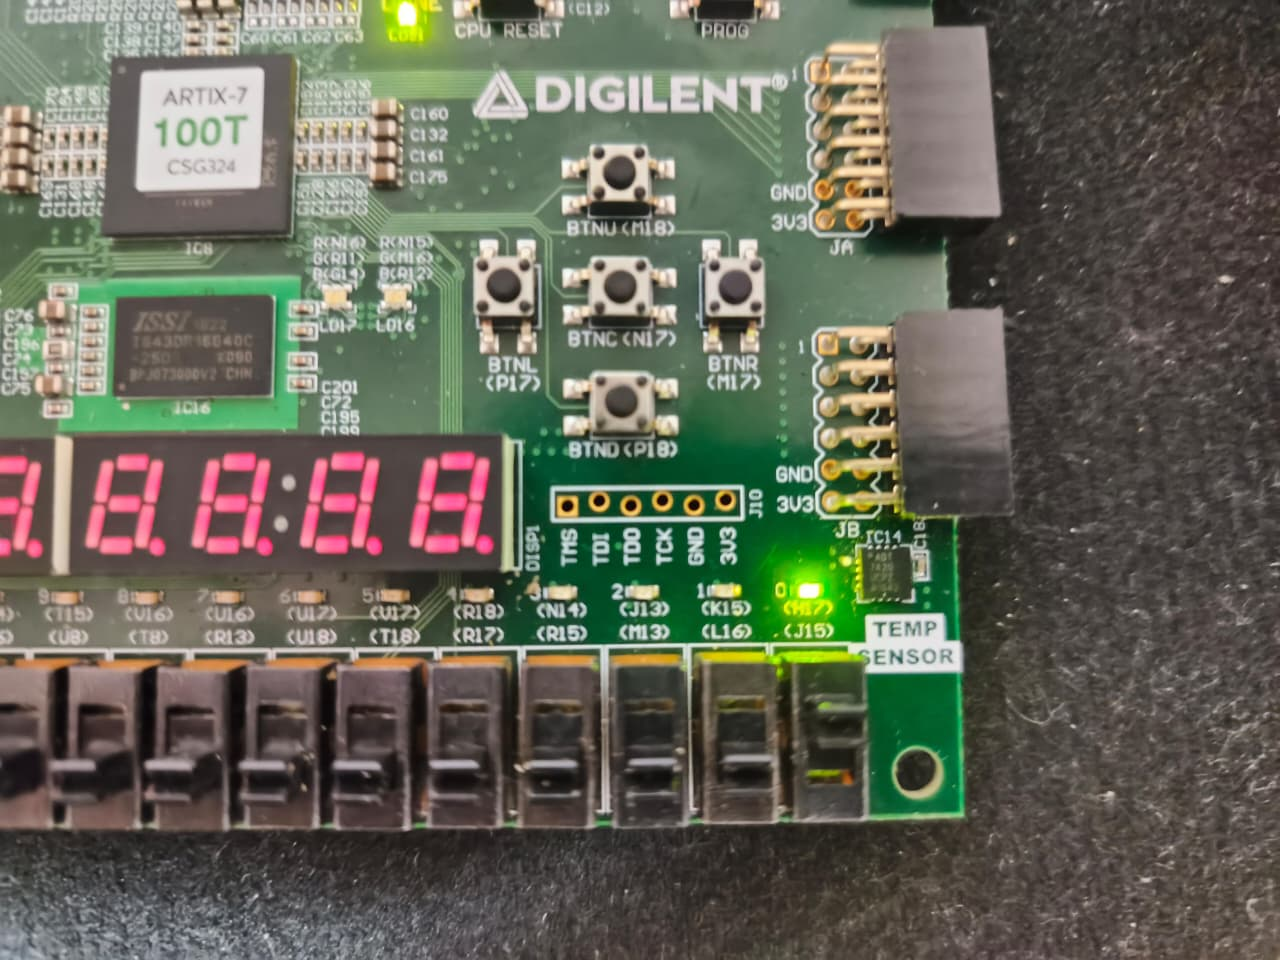
\includegraphics[width=0.6\textwidth]{Resultados/Salida_alto.jpg}
    \caption{Switch en alto: salida activa, LED encendido.}
    \label{fig:switch_alto}
\end{figure}



\end{document}
